\chapter{DistributedHElib Design} \label{chap:DistributedHElibDesign}
The second attempt at speeding up the run time of HElib utilizes a cluster of compute nodes to parallelize operations. A cluster of nodes is a connected group of machines that communicate with each other to achieve a common task. By delegating separate work to each machine, work can be split between many machines, instead of having a single machine handle the entire work load. By doing this, run times can decrease, especially if each node is working on completing an independent task, which helps complete an overall global task. As discussed in Section \ref{sec:HElibSerialDesign}, HElib utilizes a SIMD design, meaning that a single instruction or operation is performed over many pieces of independent data. With a distributed design then, the hope is to split the data up, send it to compute nodes, have those nodes perform the operations, and send the results back. Having each node work simultaneously on separate pieces of the data, can allow for a speedup in run time compared to only having a single machine work on all the data.

For this design, a master-slave architecture was chosen. This means that there will be one node, the dispatcher node, which controls the other nodes, the compute nodes. The dispatcher node will be running HElib and when needed, will assign work to the compute nodes. There are a few phases when executing operations in a distributed computing environment.

First the cluster must be setup, and nodes must be designated as compute or dispatcher nodes. Then the dispatcher node must assign work to the compute nodes. As part of assigning work, the dispatcher node must partition the data, and send the pieces to the respective compute nodes. The compute nodes must then perform the operations, and send the data back. Finally the dispatcher node collects all the results and stores them, before returning to regular execution. The cluster setup and work assignment phases are discussed in Section \ref{sec:NodeClusterSetup}. The partitioning of the data is discussed in Section \ref{sec:DistributedMemoryMapping}. Finally the methods by which the data are transmitted between nodes is discussed in Section \ref{sec:Concurrency}.
 
\section{Node Cluster Setup} \label{sec:NodeClusterSetup}
Upon start up of a cluster of nodes, each must be assigned a job. For this design a master-slave architecture is used. This means that one node must be designated the master node, which will be the dispatcher node, and the others are designated slave nodes, or compute nodes. The dispatcher node is the node responsible for running the serial portion of HElib, and distributing the data to the worker nodes when a distributed part of computation is reached. The compute nodes just wait for instructions from the dispatcher node, and act accordingly when given tasks.

When starting a cluster with OpenMPI, the distributed computing communication interface, each node is assigned a number, starting at $0$ through $num\_nodes - 1$. Node $0$ becomes the dispatcher node, and the others are compute nodes. The dispatcher node then returns to normal program execution, while the compute nodes wait for messages from the dispatcher node. 

When the dispatcher node reaches a point of execution that is meant to be distributed, it partitions the data (discussed in Section \ref{sec:DistributedMemoryMapping}) and assigns each compute node a piece of the data to operate on. The manner in which the dispatcher node chooses what compute node will operate on what piece of data is examined next.

\subsection{Work Assignment}
After the data has been partitioned, it must be assigned to a compute node to be operated on. The scheme used to choose the next compute node for a piece of data is round-robin scheduling. This scheme allows for an even or almost even distribution of the data across all the compute nodes. Having an even or almost even distribution means the lowest run times and the best efficiency. There are two cases to consider when determining if a distribution scheme is efficient: when there are more compute nodes than data pieces, and when there are fewer compute nodes than data pieces.

\begin{figure}[t!]
\centering
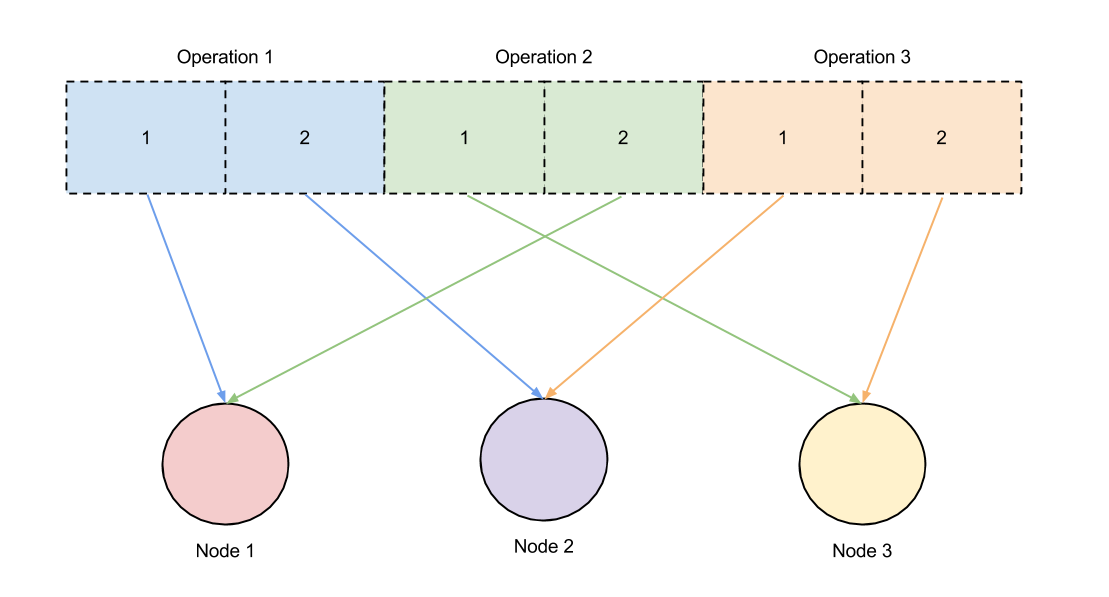
\includegraphics[width=0.95\textwidth]{RollingRoundRobinExampleMore.png}
\caption{Rolling Round Robin Example with More Nodes than Data Pieces}
\label{fig:RollingRoundRobinExampleMore}
\end{figure}
For the first case, with the round-robin scheduling, this just means that some nodes will not be working, while others are. For this design a rolling round-robin design is used. This means that for any operations, the next node to be assigned work will always be the node which was assigned work the longest time ago. This node has the highest probability of being free and ready to receive more work, compared to all the others. Figure \ref{fig:RollingRoundRobinExampleMore} shows an example of rolling round-robin scheduling applied to this case.

\begin{figure}[t!]
\centering
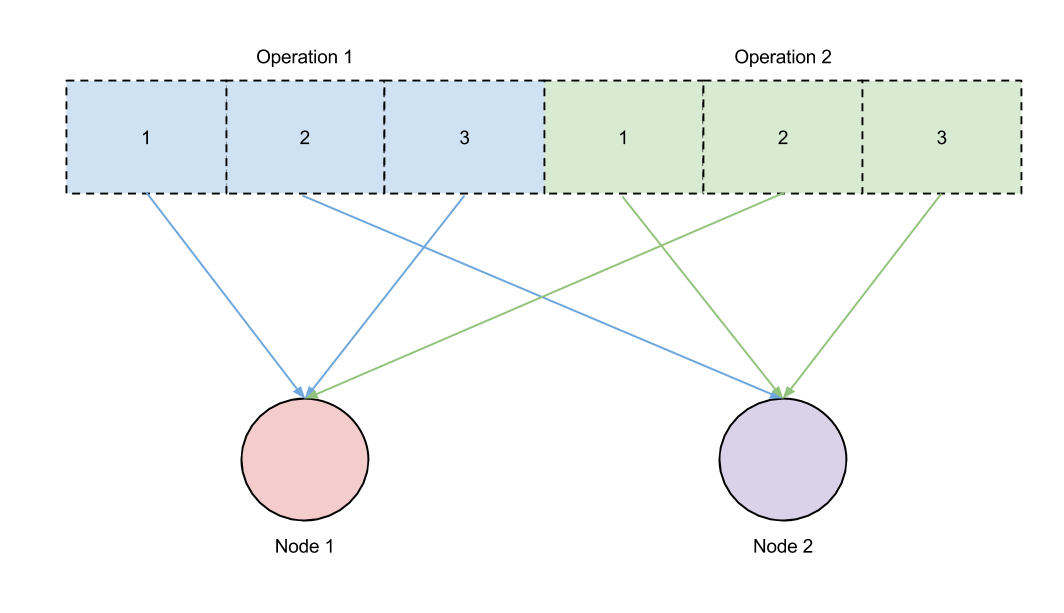
\includegraphics[width=0.95\textwidth]{RollingRoundRobinExampleLess.png}
\caption{Rolling Round Robin Example with Less Nodes than Data Pieces}
\label{fig:RollingRoundRobinExampleLess}
\end{figure}
For the second case, with the round-robin scheduling, this just means that some nodes will have multiple pieces of data to operate on. By using the round-robin scheduling though, the amount of work done by each compute node should be about equal, and thus evenly spread over the compute nodes. If work was unequally proportioned to a single compute node, compared to others, then the dispatcher node might have to wait longer for the results, before continuing normal execution. This way the greatest run time and efficiency is achieved. Figure \ref{fig:RollingRoundRobinExampleLess} shows an example of rolling round-robin scheduling applied to this case.

\section{Memory Mapping} \label{sec:DistributedMemoryMapping}
In order for the compute nodes to execute, they must have a portion of the data to work on. This requires the dispatcher node to partition the data from its current storage model into pieces, before they are sent to the compute nodes to be worked on. There are two pieces of data that need to be mapped: the data that the operation is being performed on, and the moduli.

\subsection{Mapping from Dispatcher Node to Compute Nodes}
\begin{figure}[t!]
\centering
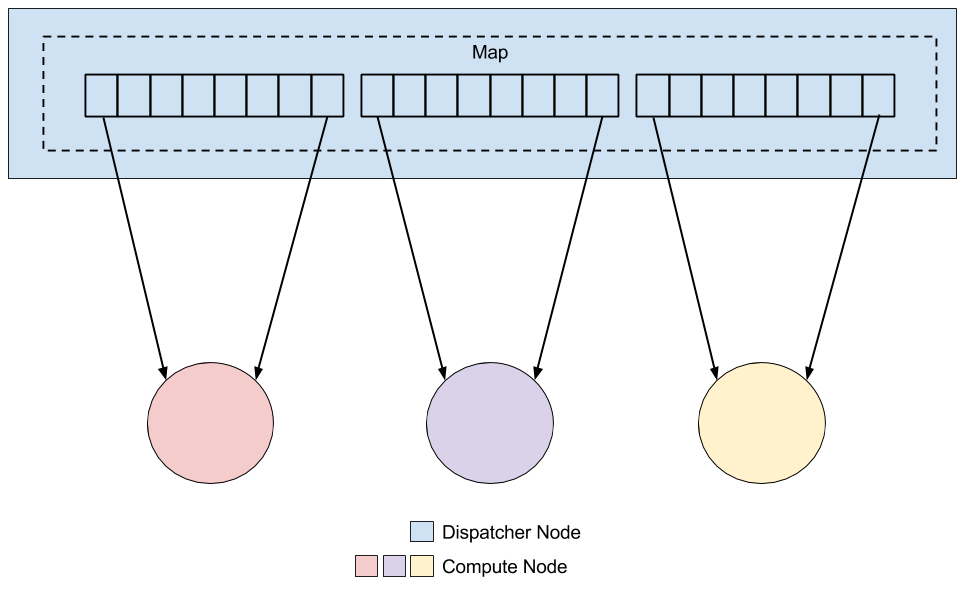
\includegraphics[width=0.65\textwidth]{MappingDispatchertoComputeData.png}
\caption{Data Mapping from Dispatcher to Compute Nodes}
\label{fig:MappingDispatcherToComputeData}
\end{figure}
Currently the data is stored as shown in Figure \ref{fig:MappingDispatcherToComputeData}. The \verb|map| contains vectors or rows, each of these rows are arrays of 64-bit integers. The rows present a great partitioning point. Splitting the data up by these rows, and sending individual rows to each compute node to be operated on, is the logical splitting point because there will always be about the same number of rows during execution, whereas the size of the rows might change often. Also, splitting rows up would cause more communication between the nodes, which could slow down run times. 

\begin{figure}[t!]
\centering
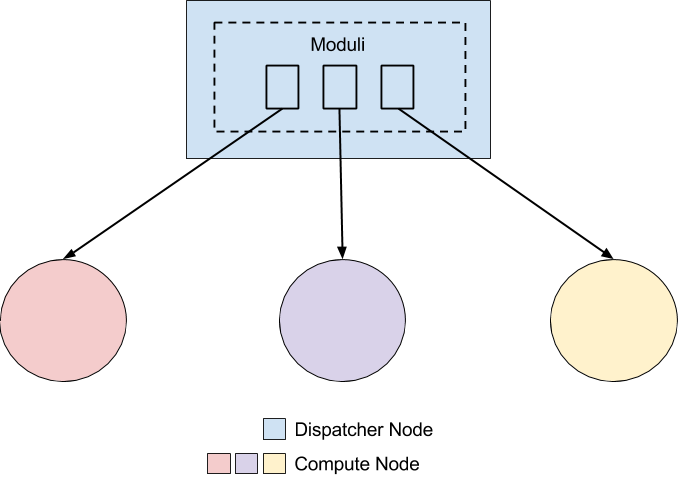
\includegraphics[width=0.65\textwidth]{MappingDispatchertoComputeModuli.png}
\caption{Moduli Mapping from Dispatcher to Compute Nodes}
\label{fig:MappingDispatcherToComputeModuli}
\end{figure}
Similarly the moduli are being stored as individual elements. Because each moduli is assigned to each row, and the rows are being assigned to a single compute node, each moduli must only be sent to the specific compute node that the row it corresponds to is on. Figure \ref{fig:MappingDispatcherToComputeModuli} shows the mapping process. Each modulus is only sent to the compute node that its corresponding row is sent to.

\subsection{Compute Node Vector Management}
Naively creating and freeing buffers on the compute nodes that will receive the data from the dispatcher node slows down run times. By creating a few buffers, and maintaining them throughout the programs lifetime, the most efficient memory usage is achieved, along with the greatest speedup.

Two buffers are created and maintained throughout the lifetime of the program. Both buffers are of size $size\_of\_row$. These are the buffers that the rows will be copied into on the compute nodes. The size, $size\_of\_row$, rarely changes, thus there will be little memory reallocation occurring. Also, reallocation will only occur when the buffer is too small, not when it is larger than needed. So the buffer will only ever grow, not shrink, thus cutting down on the occurrences of reallocation needing to be performed. The function that handles initializing and reallocation of these buffers is found in Appendix \ref{sec:ComputeNodeBufferManagement}.

\section{Concurrency} \label{sec:Concurrency}
Concurrency for a distributed system means that each node is executing operations simultaneously. To achieve concurrency in this system, the dispatcher node must be able to assign work, and not have to wait for a response, before assigning more work and the compute nodes must be able to perform computations at the same time. For all of these operations to happened concurrently, the communication between the nodes must be non-blocking.

\subsection{Non-Blocking Send and Receive with OpenMPI}
Blocking send and receive functions requires the data to be completely sent or received before continuing execution. This means that if a node were to call \verb|receive|, it would wait until it received data, before continuing execution. This can both be beneficial and detrimental, depending on the needs of the design. Non-blocking send and receive functions however schedule requests, and then continue execution. These requests will later be filled, but execution can continue, even if they have not yet been filled. So a request can be generated, and even if the data has not finished sending or been completely received, execution can continue. This request can then be tested, and once the data has been sent or received, the request will be filled. Both methods have there uses, discussed next.

\subsubsection{Send and Receive on Compute Nodes}
For the compute nodes, blocking send and receive functions are used, because it is necessary for the buffer holding the result of the operation to be sent back to the dispatcher node, before the next operation occurs. If the next operation occurred before the dispatcher node received the data, the buffer could be cleared or overwritten, and the data sent back would be incorrect.

\subsubsection{Send and Receive on Dispatcher Node}
For the dispatcher node, non-blocking send and receive functions are used. This allows the dispatcher node to continue assigning work, even if the compute nodes have not fully received their assigned work. Also the dispatcher node will use non-blocking receive functions in order to receive data back as quickly as possible. If the dispatcher node used blocking receive functions, then it could be waiting on a node that is taking a long time to perform an operation, and causing other compute nodes to wait that might have already finished computation, and may have pending computation that they could be moving onto. 

Only using non-blocking receive functions could cause problems for the dispatcher node, if for example two operations are performed, and the second requires the results from the first. Without any mechanisms to ensure the result to the first operation is received, before the execution of the second operation, unknown results can be computed. Therefore there is a need for a syncing mechanism.

\subsection{Syncing}
A syncing mechanism will cause the dispatcher node to wait for all pending requests to be completed before continuing execution. In this way, it can be ensured that a single operation is fully completed before moving onto other operations. To keep track of these requests, a queue is used. When a new request is created, through either a call to \verb|send| or \verb|receive|, it is added to the end of the queue. When the \verb|sync| function is called, each of these is tested to see if they have completed. If a request has been completed, then it is removed from the queue, if not, the function moves onto the next in the queue, and checks it. The function only returns when all the pending requests have been filled, when the queue is empty. The \verb|sync| function can be found in Appendix \ref{sec:SynchronizationManagement}. The \verb|sync| function is performed after every operation(addition, subtraction, or multiplication), to ensure that the operation has completed, before moving onto the next operation.